% vim:spelllang=uk,en
\documentclass[a4paper,notitlepage,headsepline,pdftex,oneside]{report}

\usepackage{cmap} % чтобы работал поиск по PDF
\usepackage[T2A]{fontenc}
\usepackage[utf8]{inputenc}
\usepackage[english,ukrainian]{babel}
%\usepackage{concrete}
\usepackage{cite}
\usepackage{url}
%\usepackage{pscyr}
\usepackage{textcomp}

\usepackage{textcase}
\usepackage[pdftex]{graphicx}

\usepackage{lscape}

\pdfcompresslevel=9 % сжимать PDF
\usepackage{pdflscape} % для возможности альбомного размещения некоторых страниц
\usepackage[pdftex]{hyperref}
% настройка ссылок в оглавлении для pdf формата
\hypersetup{unicode=true,
            pdftitle={PostgreSQL},
            pdfauthor={Погода Михаил},
            pdfcreator={pdflatex},
            pdfsubject={},
            pdfborder    = {0 0 0},
            bookmarksopen,
            bookmarksnumbered,
            bookmarksopenlevel = 2,
            pdfkeywords={},
            colorlinks=true, % установка цвета ссылок в оглавлении
            citecolor=black,
            filecolor=black,
            linkcolor=black,
            urlcolor=blue}

\usepackage{amsmath}
\usepackage{amssymb}
\usepackage{moreverb}
\usepackage{indentfirst}
\usepackage{misccorr}

\usepackage{xtab}
\usepackage{nccfoots}

\usepackage[left=3cm,right=2cm,top=2cm,bottom=2cm]{geometry}
\usepackage{subfig}
\usepackage{flafter}
\usepackage{caption}

\usepackage{hanging}
\usepackage{enumitem}
\usepackage{setspace}

\usepackage[rm,bf,small,raggedright]{titlesec}

\usepackage[titles,subfigure]{tocloft}

\renewcommand{\rmdefault}{ftm}
\newcommand{\setfontsize}[1]{\fontsize{#1pt}{#1pt}\selectfont}
\newcommand{\invcommas}[1]{\guillemotleft #1\guillemotright}

\binoppenalty=10000
\relpenalty=10000

\newcommand{\Chapter}[1]{\chapter{#1} \renewcommand{\baselinestretch}{1.5}\setfontsize{14pt}}
\newcommand{\uchapter}[1]{\chapter*{#1}\pagestyle{fancy}\renewcommand{\baselinestretch}{1.5}\setfontsize{14pt}\addcontentsline{toc}{chapter}{#1}}
\newcommand{\uChapter}[1]{\chapter*{#1}\pagestyle{fancy}\renewcommand{\baselinestretch}{1.5}\setfontsize{14pt}}
% для создания вступления воспользуемся командой \uchapter
\newcommand{\intro}{\uchapter{ВСТУП} \renewcommand{\baselinestretch}{1.5}}

% видоизменяем содержание
\makeatletter
\renewcommand{\tableofcontents}{%
  \begin{center}
    \textbf{ЗМІСТ}
  \end{center}

  \addvspace{10pt}
  \begin{flushright}
  \end{flushright}

  \addvspace{-15pt}

  \@starttoc{toc}
}
\makeatother

% чтобы красивые были ячейки в таблице по высоте
\renewcommand{\arraystretch}{1.2}
\setlength{\parindent}{1.25cm}

% меняем формат нумерации формул
\renewcommand{\theequation}{\arabic{chapter}.\arabic{equation}}

% новые стили для списков
% эти команды нужны для корректного отображения списков
%\renewcommand{\theenumi}{\arabic{enumi})}
%\renewcommand{\theenumii}{\arabic{enumii})}
%\renewcommand\labelenumi{\theenumi}
%\renewcommand\labelenumii{\theenumii}

% зададим новые списки, с правильным отступом
\newenvironment{enumerator}{\begin{enumerate}[leftmargin=1.6cm]%
  \setlength{\itemsep}{1pt}% команды, чтобы сделать единичный интервал в списке
  \setlength{\parskip}{0pt}
  \setlength{\parsep}{0pt}
  }{\end{enumerate}}
\newenvironment{itemizer}{\begin{itemize}[leftmargin=1.45cm]%
  \setlength{\itemsep}{1pt}% команды, чтобы сделать единичный интервал в списке
  \setlength{\parskip}{0pt}
  \setlength{\parsep}{0pt}
  }{\end{itemize}}

% специальные команды для определения длины отступа в заголовке для додатков
\newlength{\appendlength} % задаём новую единицу длины
\settowidth{\appendlength}{\hspace{1cm}\textbf{\textsc{\setfontsize{16}Додаток 1.\ }}} % отступ для Додатку

\newlength{\subappendlength} % задаём новую единицу длины
\settowidth{\subappendlength}{\hspace{1cm}\textbf{\textit{\setfontsize{14}Додаток 1.1.\ }}} % отступ для под-Додатку

% чуть больше потребуется повозиться с "Додатками"
\newcounter{append} % новый счётчик для Додатку
\setcounter{append}{0} % устанавливаем его в 0

\newcounter{subappend} % новый счётчик для секции в Додатку
\setcounter{subappend}{0} % устанавливаем его в 0

\renewcommand{\theappend}{Додаток \arabic{append}}
\renewcommand{\thesubappend}{\theappend.\arabic{subappend}} % счётчик под-Додатка должен включать счётчик Додатка

\newcommand{\append}[1]% переопределяем команды накручивания счётчиков для выведения заголовков нужного формата (см. ниже)
  {\refstepcounter{append}% накручиваем счётчик
    {\clearpage% с новой страницы
    \bfseries\setfontsize{14pt}% наш шрифт
    \begin{hangparas}{\appendlength}{1}\hspace{1cm}\theappend. #1\end{hangparas}% сам заголовок
    \vspace{24pt}% отступ
    \addcontentsline{toc}{chapter}{\theappend. #1}% и наконец вставляем в оглавление
  }
}

\newcommand{\subappend}[1]% переопределяем команды накручивания счётчиков для выведения заголовков нужного формата (см. ниже)
  {\refstepcounter{subappend}% накручиваем счётчик
    {\addvspace{12pt}% отступ
    \begin{hangparas}{\subappendlength}{1}\textbf{\textit{\setfontsize{14pt}% наш шрифт и начало абзаца с отступами
    \hspace{1cm}\thesubappend. #1}}\end{hangparas}% сам заголовок
    \vspace{12pt}% отступ
    \addcontentsline{toc}{section}{\thesubappend. #1}% и наконец вставляем в оглавление
  }
}

% теперь будем изменять стили заголовков
% сначала - для главы
\titleformat{\chapter} % указываем, что модифицируем именно главу
      {\centering\usefont{T2A}{ftm}{b}{n}\setfontsize{14pt}} % указываем формат и номера, и лейбла (жирный "все заглавные")
      {\hspace{1cm}\thechapter.} % указываем формат самого номера: число + .
      {0.5em} % расстояние между номером и лейблом
      {} % текст, предшествующий заголовку главы

% теперь - для секции
\titleformat{\section} % указываем, что модифицируем именно секцию
      {\usefont{T2A}{ftm}{b}{n}\setfontsize{14pt}} % указываем формат и номера, и лейбла (жирный)
      {\thesection.} % указываем формат самого номера: число + .
      {0.5em} % расстояние между номером и лейблом
      {} % текст, предшествующий заголовку секции

% теперь - для секции
\titleformat{\subsection} % указываем, что модифицируем именно секцию
      {\usefont{T2A}{ftm}{b}{n}\setfontsize{12pt}} % указываем формат и номера, и лейбла (жирный)
      {\thesubsection.} % указываем формат самого номера: число + .
      {0.5em} % расстояние между номером и лейблом
      {} % текст, предшествующий заголовку секции

% теперь зададим свойства абзаца
% сначала - для главы
\titlespacing{\chapter} % указываем, что модифицируем именно главу
      {2cm} % отступ слева
      {12pt} % отступ сверху
      {12pt} % отступ снизу

% теперь - для секции
\titlespacing{\section} % указываем, что модифицируем именно секцию
      {1.25cm} % отступ слева
      {6pt} % отступ сверху
      {6pt} % отступ снизу

% теперь - для подсекции
\titlespacing{\subsection} % указываем, что модифицируем именно подсекцию
      {1.25cm} % отступ слева
      {6pt} % отступ сверху
      {6pt} % отступ снизу

% переопределяем команду объявления новой секции, чтобы корректно было с полуторным интервалом
\newcommand{\Section}[1]{\section{#1} \renewcommand{\baselinestretch}{1.5}\setfontsize{14pt}}

% переопределяем команду объявления новой подсекции, чтобы корректно было с полуторным интервалом
\newcommand{\Subsection}[1]{\subsection{#1} \renewcommand{\baselinestretch}{1.5}\setfontsize{14pt}}

% теперь займёмся оглавлением
% сначала задаём расстояние между точками
\renewcommand{\cftchapdotsep}{1}
\renewcommand{\cftsecdotsep}{1}
\renewcommand{\cftsubsecdotsep}{1}

% затем - поле, выделяемое под номер страницы
\cftsetpnumwidth{1em}

% теперь займёмся главами
\renewcommand{\cftchapaftersnum}{.} % что будет писаться после номера главы
\renewcommand{\cftchapindent}{1cm} % отступ номера главы от левого края
\renewcommand{\cftchapnumwidth}{1em} % общее поле, выделяемое под номер главы
\setlength{\cftbeforechapskip}{6pt} % промежуток "до"
\renewcommand{\cftchappagefont}{\mdseries\setfontsize{14pt}} % стиль номера страницы
\renewcommand{\cftchapfont}{\mdseries} % стиль заголовка
\renewcommand{\cftchapfont}{\setfontsize{14pt}} % стиль шрифта ("все заглавные")
\renewcommand{\cftchapleader}{\cftdotfill{\cftchapdotsep}} % чем заполнять промежуток от заголовка до номера страницы (точками)

% теперь займёмся секциями
\renewcommand{\cftsecaftersnum}{.} % что будет писаться после номера секции
\renewcommand{\cftsecindent}{1.5cm} % отступ номера секции от левого края
\renewcommand{\cftsecnumwidth}{2em} % общее поле, выделяемое под номер секции
\setlength{\cftbeforesecskip}{6pt} % промежуток "до"
\renewcommand{\cftsecpagefont}{\mdseries\setfontsize{14pt}} % стиль номера страницы
\renewcommand{\cftsecfont}{\setfontsize{14pt}} % стиль шрифта
\renewcommand{\cftsecleader}{\cftdotfill{\cftsecdotsep}} % чем заполнять промежуток от заголовка до номера страницы (точками)

% теперь займёмся подсекциями
\renewcommand{\cftsubsecaftersnum}{.} % что будет писаться после номера секции
\renewcommand{\cftsubsecindent}{2cm} % отступ номера секции от левого края
\renewcommand{\cftsubsecnumwidth}{2.5em} % общее поле, выделяемое под номер секции
\setlength{\cftbeforesubsecskip}{6pt} % промежуток "до"
\renewcommand{\cftsubsecpagefont}{\mdseries\setfontsize{14pt}} % стиль номера страницы
\renewcommand{\cftsubsecfont}{\setfontsize{14pt}} % стиль шрифта
\renewcommand{\cftsubsecleader}{\cftdotfill{\cftsubsecdotsep}} % чем заполнять промежуток от заголовка до номера страницы (точками)

% заголовки таблиц и рисунков
\DeclareCaptionLabelFormat{tablecap}{Таблиця #2} % старый формат "Табл." не устраивал
\captionsetup[table]{justification=raggedleft, font={Large,rm}, textfont=md, labelsep=period, labelformat=tablecap} % сначада для таблиц
\captionsetup[figure]{justification=centering, font={Large,rm}, labelsep=period} % теперь для рисунков

% команда, изменяющая латинские буквы на привычные кириллические в подрисунках
\renewcommand{\thesubfigure}{\asbuk{subfigure}}

% теперь создадим новое окружение, сразу объединяющее в себе таблицы и "длинные" таблицы
\newenvironment{supertable}[5]{% "перед"
    \bottomcaption{#3}% заголовок таблицы
    \tablefirsthead{#5}% первый заголовок таблицы
    \tablehead{% заголовок на других страницах
        \multicolumn{#2}{l}{Продовження Табл. \thetable.}\\%
        \multicolumn{#2}{l}{}\\% красивый отступ
        #5% дописываем старый заголовок
    }
    \tabletail{\hline}% хвост таблицы
    \tablelasttail{\hline}% последний хвост таблицы
    \label{#4}% метка
    \begin{center} % открываем центрирование
    \begin{xtabular}{#1}% начнём длинную таблицу с соответствующим параметром
}
    { % "после"
    \end{xtabular} % закрываем таблицу
    \end{center} % закрываем центрирование
}

% займёмся библиографией
% меняем формат номера
\makeatletter
\renewcommand{\@biblabel}[1]{#1.}
\makeatother

% кроме того, надо добавить библиографию в оглавление
\newenvironment{references}{
  \renewcommand{\bibname}{СПИСОК ВИКОРИСТАНИХ ЛІТЕРАТУРНИХ ДЖЕРЕЛ}% меняем заголовок, показываемый при ссылках
  \begin{thebibliography}{99.}
  \addcontentsline{toc}{chapter}{СПИСОК ВИКОРИСТАНИХ ЛІТЕРАТУРНИХ ДЖЕРЕЛ}
  }
  {
  \end{thebibliography}
}

\usepackage{fancyhdr}
\renewcommand{\headrulewidth}{0pt}
\fancyhf{}
\rfoot{\thepage}

\fancypagestyle{plain}{\fancyhf{}\rfoot{\thepage}}

\pagestyle{fancy}

\usepackage{listings}
\lstloadlanguages{C++}
\lstset{language=C++,basicstyle=\scriptsize,frame=tb,commentstyle=\itshape,stringstyle=\bfseries,extendedchars=false}

\begin{document}
\setfontsize{14pt}
\renewcommand{\baselinestretch}{1.5}
\begin{titlepage}
  \begin{center}
\setfontsize{14pt}
\renewcommand{\baselinestretch}{1.5}
{\bf
    \mbox{\MakeUppercase{Міністерство освіти і науки України}}

    \mbox{\MakeUppercase{Національний технічний університет України}}

    \MakeUppercase{``Київський політехнічний інститут''}

    \vspace{2cm}


    Факультет прикладної математики

    Кафедра прикладної математики

    \vfill

    ПОЯСНЮВАЛЬНА ЗАПИСКА
  }

    зі спеціальності 6.040301 ``Прикладна математика''

    на тему:

    \textbf{Книжковий інтернет"=магазин. Робоче місце клерка}
  \end{center}

  \vfill

  \begin{minipage}{0.4\textwidth}
  \noindent
  \textbf{Студент групи} КМ-92\\
  \hspace{1cm}\\
  \noindent
  \textbf{Керівник}\\
  \end{minipage}
  \begin{minipage}{0.4\textwidth}
    \noindent
    Погода~М.\,В.\hfill\underline{\hspace{1.5cm}}\\
    \hspace{1cm}\\
    \noindent
    Терещенко~І.\,О.\hfill\underline{\hspace{1.5cm}}\\
  \end{minipage}

  \vfill

  \begin{center}
    Київ --- 2013
  \end{center}
\end{titlepage}
\uChapter{АНОТАЦІЯ}
  Дана курсова робота являє собою розробку робочого місця клерка магазину
  книжок.

  В роботі розглянуті основні обов’язки щодо підтримування актуального стану
  магазину й впровадження спеціальних пропозицій --- ,,бандлів''.

  Робоче місце клерка --- комплексне робоче місце, що має зв’язки майже з
  усіма сутностями інформаційної системи.

  Хоча клерк і супроводжує систему, але й він має обмеження: додавати нові
  книжки й видаляти ,,бандли'' може лише адміністратор.
  \clearpage
\uChapter{РЕФЕРАТ}
  \textbf{Актуальність теми.}
    За сучасних умов інформаційні системи, у складі яких зазвичай наявна деяка
    база даних, широко застосовуються.
    Ця курсова робота спрямована на здобуття вмінь в проектуванні й реалізації
    інформаційних систем та баз даних.

    В цій роботі створюється робоче місце клерка магазину книжок.
    Підтримування конкурентоспроможності магазину є актуальною темою за
    сучасних умов.

  \textbf{Об’єктом дослідження} в даній роботі є робоче місце клерка.

  \textbf{Предмет дослідження} --- організація спеціальних умов як можливість
  підвищення конкурентоспроможності магазину.

  \textbf{Мета роботи:} визначити оптимальний метод організації спеціальних
  умов та метод контролювання актуальності бібліотеки магазину.

  \textbf{Методами дослідження} даної системи було обрано \emph{кольорові
  сеті Петрі}, \emph{діаграми потоків даних}, \emph{діаграми потокового опису
  послідовності виконання етапів процесу}, \emph{діаграми послідовності зміни
  станів об’єктів} та \emph{діаграми взаємозв’язків сутностей}.

  \textbf{Наукова новизна} роботи полягає у створенні окремого робочого місця
  для людини, що слідкує за актуальністю стану бібліотеки магазину й створенні
  системи спеціальних умов на базі ,,бандлів''.

  \textbf{Практична цінність} отриманих в роботі результатів полягає в тому,
  що запропоновані методи та засоби дають змогу підтримувати актуальність
  стану бібліотеки магазину й підвищувати конкурентоспроможність магазину за
  допомогою системи спеціальних пропозицій.

  \textbf{Апробація роботи.}
  Дана робота була випробувана на побудові моделі інформаційної системи
  інтернет"=магазину книжок.

  \textbf{Структура та обсяг роботи.}
    Курсова робота складається зі вступу, 5 розділів та висновків.

    \emph{У вступі} надано загальну характеристику роботи.

    \emph{У першому розділі} розглянуте передпроектне дослідження ІС.

    \emph{У другому розділі} проаналізовані задачі й цілі курсової роботи.

    \emph{У третьому розділі} проаналізовані основні сутності ІС та їх
    зв’язки.

    \emph{У четвертому розділі} проаналізовані зв’язки між усіма сутностями, з
    якими повинен працювати клерк.

    \emph{У п’ятому розділі} проаналізовані основні бізнес"=процеси, що
    відбуваються у даній підсистеми ІС.

    \emph{У висновку} проаналізовані отримані результати роботи.
%TODO:
    Робота виконана на $N$ аркушах, містить посилання на список використаних
    літературних джерел з 4 найменувань.
    У роботі наведено 5 рисунків та 1 таблиця.

  \textbf{Ключові слова:} робоче місце клерка, система спеціальних пропозицій,
  система знижок, ,,бандли''.
  \clearpage
\tableofcontents
\clearpage
\uchapter{СПИСОК ТЕРМІНІВ, СКОРОЧЕНЬ ТА ПОЗНАЧЕНЬ}
  \begin{itemizer}
    \item[] \emph{ІС} --- інформаційна система.
    \item[] \emph{ERD} --- Entity-Relationship Digram.
    \item[] \emph{DFD} --- Data Flow Diagram.
    \item[] \emph{PFDD} --- Process Flow Description Diagrams.
    \item[] \emph{IDEF3} --- Integrated DEFinition for Process Description Capture
      Method.
    \item[] \emph{OSTN} --- Object State Transition Network.
    \item[] \emph{т.\,д.} --- так далі.
  \end{itemizer}
  \clearpage
\intro
  Внаслідок нестримного збільшення користувачів глобальної мережі, кількість
  можливих покупців електронного товару також зростає.

  Електроні магазини не потребують орендування приміщень, не потребують
  працівників"=консультантів, а тому є більш економічно вигідним.

  Електроні магазини розширюють ринки збуту, в той же час розширюються й
  можливості покупців, а тому, згодом, можна буде купувати будь"=який товар в
  будь"=який час в будь"=якій країні.
  Це дає електронним магазинам вагому перевагу над звичайними.

  Глобалізація інтернету зробили електронну комерцію можливою для підприємств
  будь"=якого масштабу.

  Сьогодні виробники та продавці можуть легко переходити від ,,звичайної''
  торгівлі до ,,електроної''.

  Для актуалізації стану магазину потрібно вчасно поповнювати запаси магазину
  або створювати попит на книги через деякі спеціальні пропозиції.
  Саме таке робоче місце й було розроблене під час виконання цієї курсової
  роботи.
\Chapter{АНАЛІЗ ПІДПРИЄМСТВА АВТОМАТИЗАЦІЇ}
  \Section{Межі проекту}
    Проект має перед собою мету автоматизувати частину роботи
    інтернет"=магазину книжок, а саме роботу клерка --- особи, відповідальної
    за наявність книжок у сховищах, актуальність існуючих ,,бандлів'',
    своєчасність повернення орендованих книжок, тощо.

    У багатьох існуючих проектах ці обов’язки розосереджені між різними
    працівниками, але, якщо об’єднати ці обов’язки у межах обов’язків однієї
    людини, можна покращити актуальність й своєчасність реагування на ті чи
    інші події.
    Розвиток інформаційних технологій не повинен якось сильно вплинути на
    розроблене робоче місце клерка.
    Завдяки розвитку можливе тільки прискорення роботи.

    Рішення, що ми матимемо завдяки цьому проекту, повинно бути актуальним
    протягом наступних десяти років.
    Можливе лише скорочення числа обов’язків клерка, адже із розвитком
    інформаційних технологій електронна література виходить на передній план,
    a тому, наприклад, слідкувати за наявністю книжок на сховище не
    знадобиться.
  \Section{Бізнес"=потреби}
    Насамперед треба зазначити, що цей проект повинен буде працювати у сфері
    обслуговування користувачів, а тому

    Для успішного функціонування проекту необхідно використовувати будь"=яку
    ЕОМ під управлінням операційних систем на базі UNIX або
    Microsoft Windows.

  \Section{Безпека}
    Оскільки клерк повинен працювати майже з даними, що є в інформаційній
    системі, це робоче місце є критичним.

    Клерк може вплинути як на ціну нових ,,бандлів'', так і змінити ціну
    існуючих.

    Очевидно, що правила безпеки для цього робочого місця повинні бути
    підвищеними.
    Це повинні бути як певні політики безпеки, так і аудит.
    Додатково можна зазначити, що окрім звичайної політики щодо наявності
    доступу лише до таблиць, з якими клерк має працювати, треба перекласти
    значну частину правил у ,,бізнес"=логіку''.
  \Section{Продуктивність}
    Під продуктивністю клерка, а й отже і усього магазину, треба
    усвідомлювати наскільки швидко клерк може виконувати свої обов’язки у цій
    системі.
    Продуктивність системи може бути виміряною згідно багатьох факторів.
    Але як саме ці фактори можуть впливати на продуктивність системи, залежить
    від архітектури рішення та від того, як воно було спроектоване.

    Аналізуючи потреби продуктивності треба розуміти наступне:
    \begin{itemizer}
      \item кількість транзакцій за одиницю часу;
      \item пропускну здатність;
      \item потужність системи;
      \item перешкоди продуктивності;
      \item взаємодія з існуючими стандартами;
      \item бажаний час відповіді під сервера.
    \end{itemizer}
  \Section{Супровід}
    Супроводом всієї загальної інформаційної системи займається саме
    \emph{Clerk} (робота з боржниками, слідкування за актуальністю цін на
    книжку, поповнення ,,бандлів'', тощо).

    Також супроводжує систему \emph{Admin}, який додає нові книжки до системи,
    реєструє нових користувачів та працівників, тощо.
  \Section{Людський фактор}
    Робоче місце клерка цієї інформаційної системи орієнтоване на користувачів
    віком від 18 років.

    Хоча інтерфейс є інтуїтивно зрозумілі, але користувачі потребують
    додаткового навчання, адже їх обов’язки не є тривіальними.

    Особою, що повинна буде працювати за цим робочим місцем, повинна бути
    орієнтуватися у тому, яки книги починають користуватися попитом, а тому їх
    можна об’єднати у ,,бандли'', а також вміти користуватися ЕОМ на рівні
    звичайного користувача.
  \Section{Розширюваність}
    Система є досить гнучкою щодо росту покупців, клерків, книжок у наявності.

    Але система дозволяє магазину реалізовувати лише книжки.
  \Section{Методології}
    Для проектування інформаційної системи можуть використовуватись наступні
    методології:
    \begin{enumerator}
      \item ERD
      \item DFD
      \item IDEF3
      \item Матриці подій.
      \item Кольорові сеті Петрі.
    \end{enumerator}
  \clearpage
\Chapter{ПОСТАНОВКА ЗАДАЧІ}
  Створити підсистему інформаційної системи ,,Книжковий інтернет"=магазин'',
  яка являє собою робоче місце клерка, що супроводжує магазин.

  Тобто необхідно спроектувати та реалізувати частину загальної
  ІС --- додаток для клерка.

  \Section{Категорії користувачів}
    Дана підсистема створена для використання працівниками магазину ---
    \emph{клерками}.

    Клерк займається слідкуванням за актуальністю цін на книги, слідкує за
    попитом на певні видання й створює ,,бандли''.
  \Section{Класи даних}
    Клерк має доступ майже до усіх сутностей інформаційної системи:
    \begin{itemizer}
      \item книги;
      \item книги, що були:
        \begin{itemizer}
          \item переглянуті,
          \item замовлені,
          \item орендовані;
        \end{itemizer}
      \item ,,бандли'';
      \item заявки адміністратору на поповнення бібліотеки.
    \end{itemizer}
    \clearpage
  \Section{Матриця подій}
    \begin{supertable}{|c|p{0.3\textwidth}|p{0.11\textwidth}|p{0.37\textwidth}|}{4}{Матриця подій (ELM)}{table:elm}
      \hline
      \bf\No &\bf Опис події &\bf Тип події &\bf Реакції на подію\\
      \hline\hline
      1 & Клерк оцінює попит на товар & N & Надати клерку доступ до таблиць
      \texttt{Books}, \texttt{History of Purchasing}\\
      \hline
      2 & Клерк додає bundle & N & Надати клерку форму для введення назви
      bundle та індивідуальних знижок для кожної книги у його складі, виконати
      відповідне додавання у таблиці \texttt{Bundle} та \texttt{BundledBook}\\
      \hline
      3 & Клерк видаляє книгу/bundle & NN & Звернутися до адміністратору ІС\\
      \hline
      4 & Клерк змінює інформацію щодо книги/bundle & NN & Звернутися до
      адміністратору ІС\\
      \hline
      5 & Клерк створює запит щодо поповнення запасу книг & N & Надати форму
      для вибору необхідної кількості, виконати відповідні додавання у таблиці
      \texttt{Request}\\
      \hline
    \end{supertable}
  \Section{Бізнес"=правила}
    Насамперед, можна зазначити наступні обов’язки клерка, які це рішення
    повинно дозволити виконувати:
    \begin{itemizer}
      \item Контролювати кількість книжок у сховищі.
      \item Контролювати актуальність цін на книжки.
      \item Слідкувати за попитом й керувати їм завдяки створенню ,,бандлів''
        --- сукупністю книжок, купуючи яку покупець отримує зазначену знижку
        на кожну з книжок.
      \item Слідкувати за своєчасним поверненням орендованих книжок.
    \end{itemizer}

    Клерк має можливість:
    \begin{itemizer}
      \item переглядати розгорнути інформацію про історію переглядів,
        замовлень книжок;
      \item переглядати список боржників (покупців, що затримують орендовану
        книгу понад час на який вони її орендували);
      \item створювати новий ,,бандл'' й наповнювати його книжками, вказуючи
        окрему знижку для кожної книжки у складі цього ,,бандлу'';
      \item створювати заявку адміністратору (робоче місце \emph{Admin}) щодо
        поповнення бібліотеки.
    \end{itemizer}
  \clearpage
\Chapter{ІНФОЛОГІЧНЕ ПРОЕКТУВАННЯ}
  \Section{Визначення сутностей}
    \begin{itemizer}
      \item \emph{Clerk} --- ім’я, контактна інформація.
      \item \emph{Book} --- інформація про книгу, її вартість, кількість на
        складі.
      \item \emph{Bundle} --- назва ,,бандлу''.
      \item \emph{BundledBook} --- власна знижка книжки у конкретному
        ,,бандлі''.
      \item \emph{History of Browsing} --- історія перегляду книжок
      \item \emph{Rented Book} --- книжки, що були орендовані.
      \item \emph{Customer} --- ім’я, контактна інформація.
      \item \emph{Request} --- скільки треба замовити конкретної книжки у
        постачальників.
    \end{itemizer}

  \Section{Визначення зв’язків між сутностями}
    \begin{figure}[h]
      \centering
      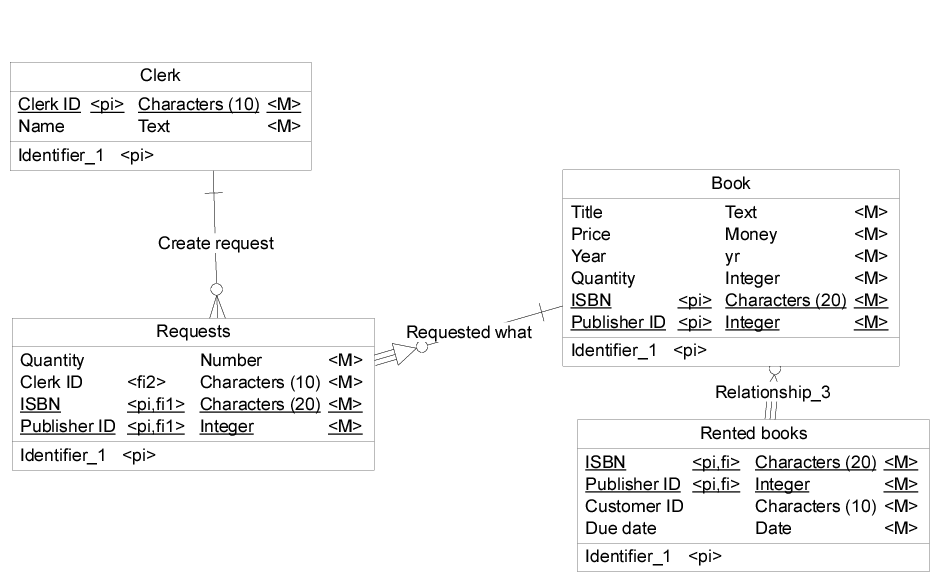
\includegraphics{small_erd.png}
      \caption{Зв’язки із головною сутністю}
      \label{fig:small-erd}
    \end{figure}
  \clearpage
\Chapter{ДАТАЛОГІЧНЕ ПРОЕКТУВАННЯ}
  \Section{Entity-Relationship Diagram}
    \begin{figure}[h]
      \centering
      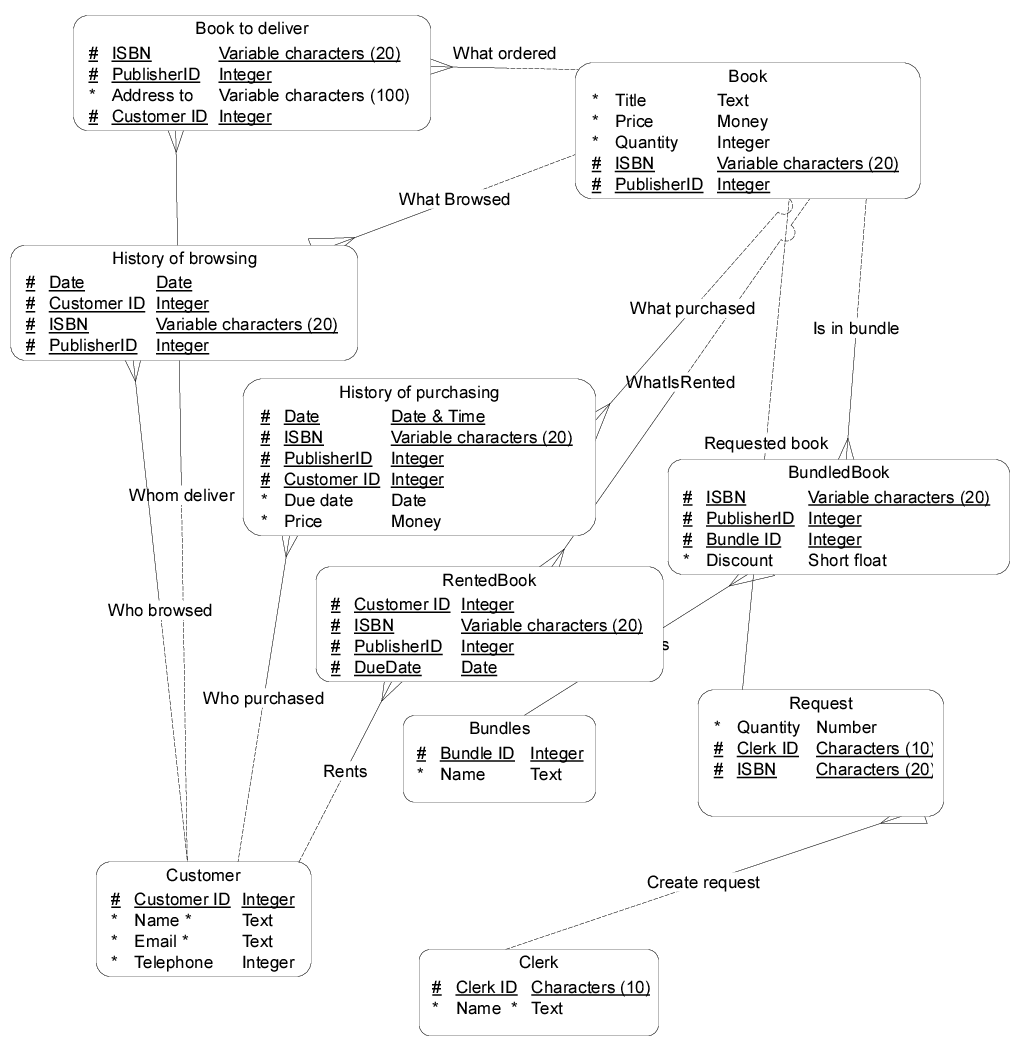
\includegraphics{big_erd.png}
      \caption{Діаграма зв’язків між сутностями}
      \label{fig:erd}
    \end{figure}
  \clearpage
\Chapter{МОДЕЛЮВАННЯ БІЗНЕС"=ПРАВИЛ}
  \Section{Data Flow Diagram}
    \begin{figure}[h]
      \centering
      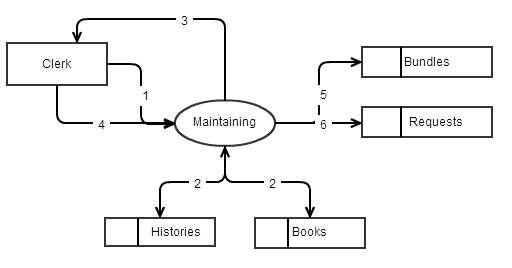
\includegraphics{dfd.png}
      \caption{Діаграма потоку даних для клерка}
      \label{fig:dfd}
    \end{figure}
    \begin{enumerator}
      \item Клерк ініціює процес супроводження ІС.
      \item Отримування даних з історій покупки/перегляду книжок та даних про
        наявність книжок на складі.
      \item Відображення усієї необхідної інформації клерку.
      \item Клерк приймає рішення щодо створення ,,бандлу''/запиту на нові
        книжки.
      \item Створюються ,,бандл'', обраний клерком.
      \item Створюються запроси адміністратору щодо поповнення бібліотеки.
    \end{enumerator}
    \clearpage
  \Section{IDEF3}
    \Subsection{PFDD}
      \begin{figure}[h]
        \centering
        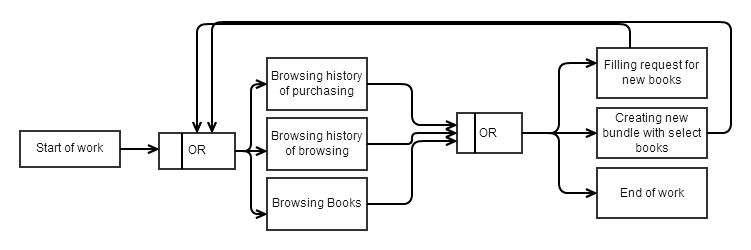
\includegraphics[scale=0.6]{pfdd.png}
        \caption{Діаграма потокового опису послідовності виконання етапів
        процесу}
        \label{fig:pfdd}
      \end{figure}
    \Subsection{OSTN}
      \begin{figure}[h]
        \centering
        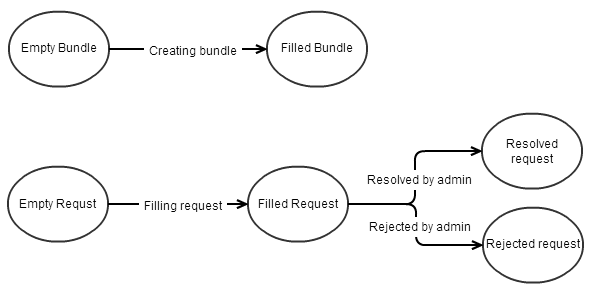
\includegraphics[scale=0.6]{ostn.png}
        \caption{Діаграма послідовності зміни стану об’єкта}
        \label{fig:ostn}
      \end{figure}
      \clearpage
\Chapter{ВИКОРОСТОВНІСТЬ}
  При побудові графічного інтерфейсу користувача (GUI) дуже важливу роль грає
  юзабіліті цього самого інтерфейсу.
  \emph{Юзабіліті} ---  поняття в мікроергономіці, що визначає загальну
  степінь зручності предмета при використанні.

  При проектуванні цього програмного продукту використовувався принцип ,,Усе,
  що користувач не може зробити повинно бути схованим''.
  Завдяки цьому прийому у користовача не повинно виниканити питання, чому та
  чи інша дія не доступна зараз.

  Заради цього актуальність стану усіх віджетів контролюється при кожній
  взаємодії з користувачем.
  \clearpage
  \Section{Граф інтерфейсу}
    \begin{figure}[h]
      \centering
      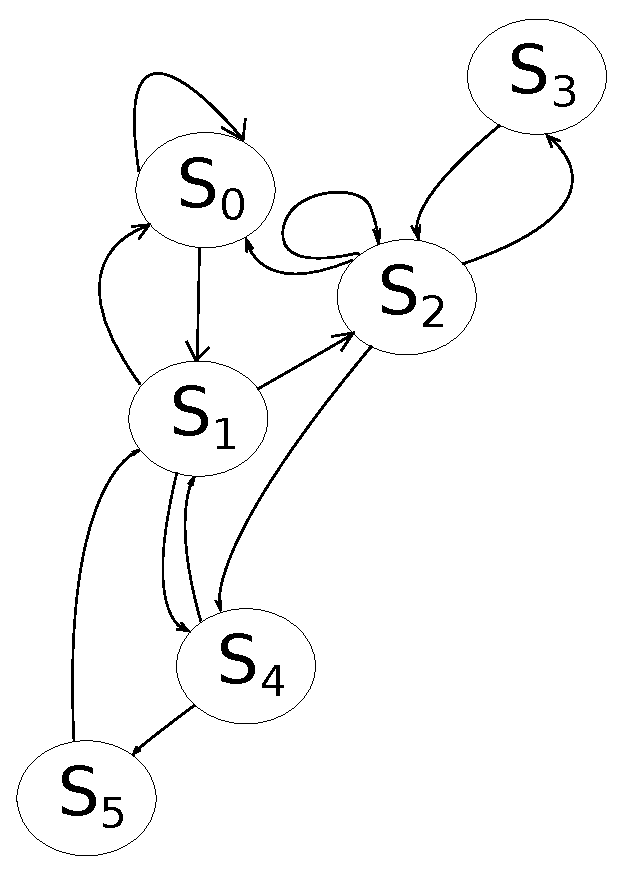
\includegraphics{gui-graph.eps}
      \caption{Граф поведінки меню}
      \label{fig:graph-gui}
    \end{figure}
    \begin{supertable}{|p{3em}|p{7em}|p{8em}|p{10em}|p{3em}|}{5}{Таблиця
      поведінки в меню}{table:guigraph}
      \hline
      \multicolumn{3}{|c|}{Стан} & \multicolumn{2}{|c|}{Перехід}\\
      \hline
      Познач. & Назва & Дія & Умова переходу & Наст. стан\\
      \hline
      $S_0$ & Вхід в систему & Клерк бажає залогінитись & Логін та пароль
      введені вірно & $S_1$\\
      \cline{4-5}
      & & & Логін чи пароль уведені невірно & $S_0$\\
      \cline{3-5}
      & & Клерк бажає вийти з програми & Натиснуто ,,Вихід'' & --\\
      \hline
      $S_1$ & Вікно пошуку книг & Клерк бажає разлогінитись & -- & $S_0$\\
      \cline{3-5}
      & & Клерк бажає обрати рядок & Присутній рядок у таблиці & $S_2$\\
      \cline{3-5}
      & & Клерк бажає перейти я друге вікно програми & Бандл повинен
      створюватись у цей момент & $S_4$\\
      \hline
      $S_2$ & Вікно пошуку книг із обраним рядком & Клерк бажає разлогінитись &
      -- & $S_0$\\
      \cline{3-5}
      & & Клерк бажає додати запит на нову постачу книжок & У системі не
      повинно бути інших запитів на цю книжку & $S_3$\\
      \cline{3-5}
      & & Клерк бажає змінити або видалити існуючий запит & Запит, що існує у
      системі, повинен бути створений цим клерком & $S_3$\\
      \cline{3-5}
      & & Клерк бажає додати книжку до бандлу, що створюється & Бандл повинен
      створюватись й там не повинно бути цієї книжки & $S_2$\\
      \cline{3-5}
      & & Клерк обирає інший рядок & -- & $S_2$\\
      \hline
      $S_3$ & Форма створення або модифікація запитів на нові книжки & Клерк
      закриває цю форму & -- & $S_2$\\
      \hline
      $S_4$ & Вікно створення бандлу & Клерк бажає перейти у друге вікно
      програми & -- & $S_1$\\
      \cline{3-5}
      & & Клерк бажає зберегти бандл & -- & $S_1$\\
      \cline{3-5}
      & & Клерк обирає якусь книжку з бандлу, що створюється & Повинна бути
      книжка в цьому бандлі & $S_5$\\
      \hline
      $S_5$ & Вікно створення бандлу із обраною книжкою & Змінити знижку цієї
      книжки & -- & $S_5$\\
      \cline{3-5}
      & & Клерк бажає перейти у інше вікно програми & -- & $S_1$\\
      \hline
    \end{supertable}
    \clearpage
  \Section{Інструкція для користувача}
    Після запуску програми, з’явиться форма логіну (див.
    рис.~\ref{fig:loginform}), в яку потрібно ввести логін і пароль до існуючої
    облікового запису клерка.
    Якщо були вказані невірні дані, то з’явиться діалогове вікно з запитом
    щодо введеня даних знову.
    \begin{figure}[h]
      \centering
      
\includegraphics{loginform.png}
      \caption{Форма логіну}
      \label{fig:loginform}
    \end{figure}

    Під час роботи завжди наявні меню для виходу з систему, (пере)входу або
    заверешення роботи з додатком.

    Після успішного входу в систему відбудеться зчитування інформації у
    таблицю, що містить книжки, з якими може оперувати клерк.
    (див.~рис.~\ref{fig:mainformtab1})
    \begin{figure}[h]
      \centering
      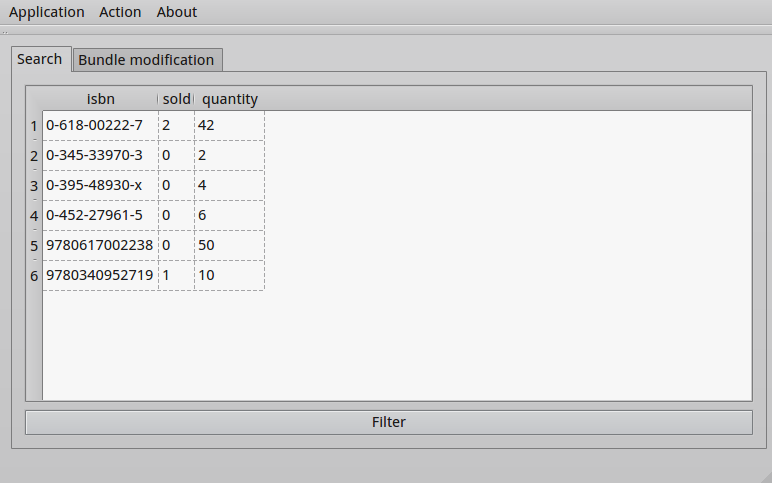
\includegraphics[width=\textwidth]{mainformtab1.png}
      \caption{Початкова форма додатку}
      \label{fig:mainformtab1}
    \end{figure}

    Для того, щоб змінити метод фільтрації, потрібно нажати на кнопку
    ,,Filter'', після чого зв’явиться віджети контролювання фільтрацію
    (див.~рис.~\ref{fig:filter}).
    За допомогою їх можна як обрати тільки ті книжки, що або погано продаються
    (,,Overstocked''), або навпаки (,,Trending''), так і створити власний
    пошук (,,Custom'').
    \begin{figure}[h]
      \centering
      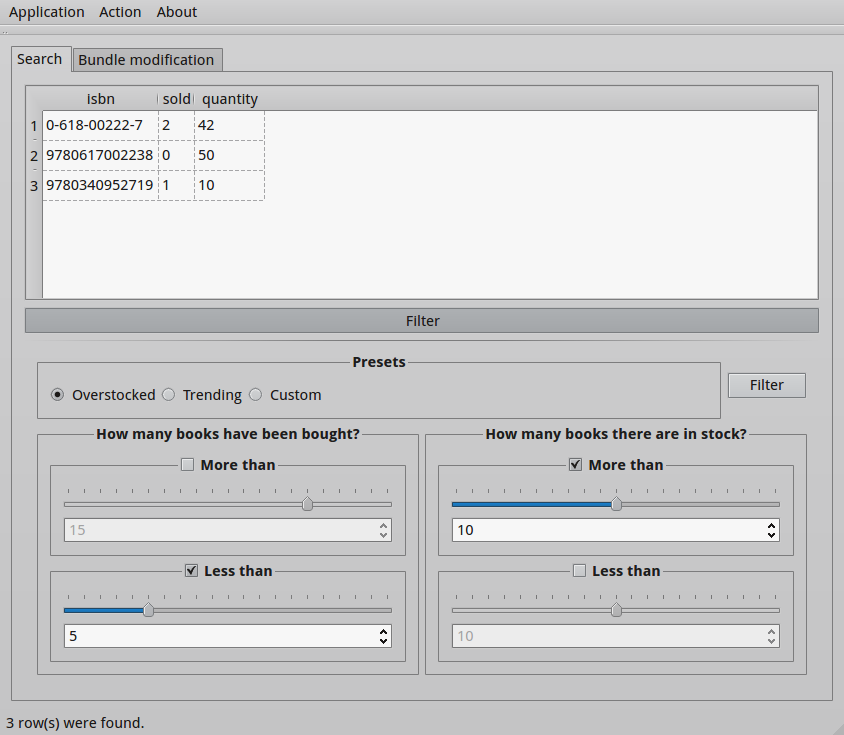
\includegraphics[width=\textwidth]{filter.png}
      \caption{Активована форма фільтрації}
      \label{fig:filter}
    \end{figure}

    Якщо користувач обирає якусь книгу з таблиці, то відобразиться форма, на
    якій буде доступна детальна інформація щодо цієї книги.
    Також, при кожному виборі книги список доступних дій змінюється як того
    потребує бізнес"=логіка.

    Для додавання запиту щодо поповнення запасу книг клерк повинен натиснути
    кнопку ,,Fill Request''.
    Для того, щоб змінити або видалити свій попередній запит, він може нажати
    ,,Modify Request'' або ,,Remove request''.

    Для того, щоб почати створювати бандл достатньо нажати ,,Add to Bundle'',
    після чого книжку будуть додаватися до віртуальної таблиці, що містимеме
    усі книжки, що повинні бути в цьому бандлі (див.~рис.~\ref{fig:Bundle}).
    \begin{figure}[h]
      \centering
      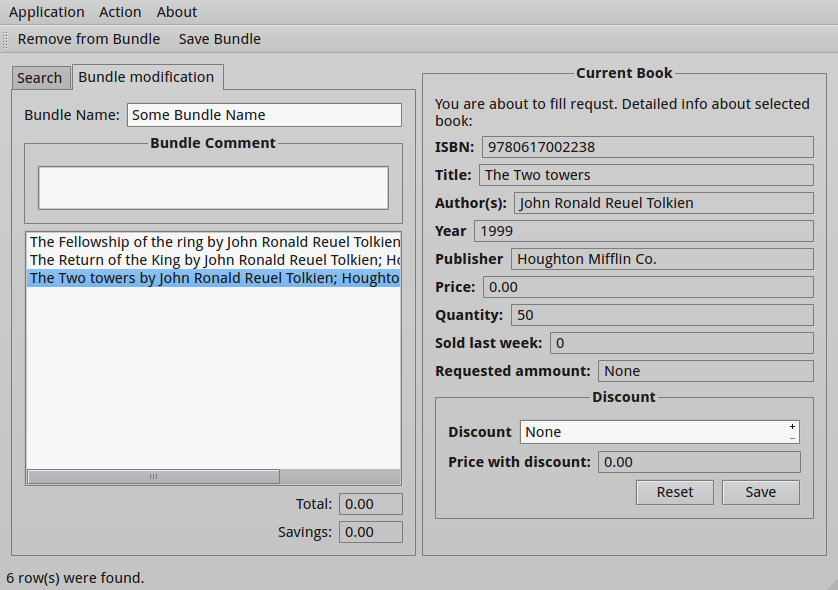
\includegraphics[width=\textwidth]{bundle.png}
      \caption{Вікно створення бандлу}
      \label{fig:bundle}
    \end{figure}

    Клерк може змінити назву або опис бандлу, а також іднивідуальні знижки на
    кожну з книжок у бандлі.

    Для збереження бандлу у базу даних достатньо натиснути ,,Save Bundle''.

\Chapter{ПРОГРАМНА РЕАЛІЗАЦІЯ}
  Для створення і збереження бази даних використовується СУБД Oracle DBMS 11g.
  Програма-клієнт «Книжковий магазин. Клерк» написана на платформі Qt 4.8 з
  використанням мови програмування C++.

  СУБД Oracle була обрана з наступних причин:
  \begin{itemize}
    \item Синтаксис близький до стандарту (порівняно з MySQL);
    \item Об'єктно"=орієнтований підхід;
    \item Check constraints;
    \item Робота з великою кількістю підключень
  \end{itemize}

  Qt дозволяє створювати платформо-незалежні програми для роботи з базами
  даних, використовуючи стандартні СУБД (якщо для яких існують рідні
  драйвери).
  Також Qt забезпечує легку роботу з запитами та їх виведенням за допомогою
  класів QSqlQuery та QSqlQueryModel, що являють собою класи з MVC-фреймворка
  Qt.

  MVC дозволяє відокремити внутрішнє представлення даних від їх відображення.

  Підключення програми до бази даних відбувається за допомогою драйвера QOCI.

  \Section{Системні вимоги}
    Основні вимоги щодо розроблюваного доданку диктуються СУБД Oracle.
    Для самого доданку необхідно будь"=яка система з 20--40 МіБ ОЗУ й вільного
    міста на жорсткому дискі.

    Оскількі в розробці використовувався фреймворк Qt, цей доданок може
    використовуватись на широкому розмаїтті операційних систем: GNU/Linux,
    MacOS X, Windows, тощо.
  \Section{Функції}
    Уся логіка розроблюваного доданку знаходиться безпосередньо у коді цього
    доданку (тобто не використовуються процедурний язик СУБД Oracle).

    Повний перелік методів й класів, що працюють з базою даних:
    \begin{itemize}
      \item \verb'struct DBOpener' --- допоміжний \texttt{RAII}-клас, що
        дозволяє автоматично закривате підключення, що було відкрите.
      \item \verb'QSqlQueryModel *m_inputModel' --- модель (внутрішнє
        представлення результату SQL-запиту.
      \item \verb'void MainWindow::setupConnection()' --- метод, що налаштовує
        підключення до серверу бази даних, зчитуючи необхідні опції з файлу
        опцій \texttt{settings.ini}.
      \item \verb'const QStringList findAuthorsForBook( const QString& isbn )'
        --- метод, що повертає список авторів, що написали книжку з заданим
        номером ISBN.
      \item \verb'void MainWindow::modifyRequest()' --- метод, що обробляє
        запит користувача на зміну попередньо"=створеного запиту на поповнення
        запасу книг.
      \item \verb'void MainWindow::removeRequest()' --- метод, що обробляє
        запит користувача на видалення попередньо"=створеного запиту на
        поповнення запасу книг.
      \item \verb'void MainWindow::fillRequest()' --- метод, що обробляє
        запит користувача на створення запиту на поповнення запасу книг.
      \item \verb'void MainWindow::saveBundle()' --- метод, що зберігає бандл
        разом з його книжками до бази даних.
    \end{itemize}
  \Section{Оптимізація}
    Під час попереднього проектування й дослідження було виявлено, що з такою
    структурою бази даних, абсолютна більшість запитів порівнюють лише поля,
    що є ключами у відповідних таблицях, а отже автоматично"=згенерованих
    індексів буде достатньо.

    Для прискорення роботи кожного запиту було досліджено, які саме поля
    найчастіше будуть відрізнятись, а тому їх слід ставити першими у логічному
    виразу, що складається лише з логічних І.
    Наприклад, у багатьох таблицях дата замовлення є частиною складеного
    первинного ключа, але вони, скоріш за все, будуть різниться у двох окремо
    взятих записах, а тому перевірку на рівність цієї дати треба ставити
    першою.

    Також для прискорення роботи бандл, що створюється, зберігається лише в
    внутрішньому стані доданку й записується до бази даних лише після усіх
    змін.

    Оскільки з’єднання з базою даних може бути досить дорогим, воно не
    тримається відкритим довше ніж того потребує ситуація.
    \clearpage
\Chapter{БЕЗПЕКА}
  Перш за все, заради того, щоб зловмисник не був у змозі викрасти паролі
  користувачів, вони зберігаються у вигляді хешсум.
  При такій організації, якщо ж все-таки зловмисник проникне у базу даних, він
  не зможе дізнатися паролю користувачів.

  Для покращення безпеки, усі додатки для клерка повинні використовувати, по
  можливості, лише один акаунт, у якого були б лише мінімальні права на
  таблиці й базу даних взагалом.

  А саме, у цього користувача повинні бути права на читання, запис та
  видалення з таблиці \texttt{request}, на запис й читання з таблиць:
  \begin{itemize}
    \item \texttt{bundle}
    \item \texttt{bundledbook}
    \item \texttt{clerk}
  \end{itemize},
  й права лише на читання з таблиць:
  \begin{itemize}
    \item \texttt{author}
    \item \texttt{book}
    \item \texttt{book\_s\_author}
    \item \texttt{customer}
    \item \texttt{history\_of\_purchasing}
    \item \texttt{publisher}
  \end{itemize}

\uchapter{ВИСНОВКИ}
  В результаті виконаної роботи було зпроєктовано підсистему ІС
  ,,Інтернет"=магазин книжок'' --- робоче місце клерка.

  Ця підсистема є підсистемою супроводу магазину, основною метою якої є
  забезпечення конкурентоспроможності магазину.

  Вирішена поставлена задача є гарним прикладом системи спеціальних
  пропозицій, адже така система може бути застосована до будь"=якого магазину.
  Але друга частина обов’язків клерка --- слідкування за наявностю популярних
  книжок у бібліотеці магазину --- скоріш за все стане не актуальною протягом
  наближчих 5--10 років.

  Як було зазначено, дана система має досить суттєве значення в сфері
  обслуговування користувачів.
  \clearpage
\begin{references}
  \item Додаткові розділи БД та ІС [Текст]: методичні
    вказівки/Л.\,О.~Ковальчук"=Хімюк, І.\,О.~Терещенко.
  \item Матриця подій [Електронний ресурс]. --- Режим доступу:
    \url{http://mathematics.is-great.org}
  \item Аналіз бізнес потреб [Електронний ресурс]: лекція/І.\,О.~Терещенко.---
    Режим доступу: \url{http://mathematics.is-great.org}
  \item Дипломне проектування за напрямами підготовки ,,Прикладна
    математика'', ,,Комп'ютерна інженерія'', ,,Програмна інженерія''
    [Текст]:навч."=метод. посіб./Є.\,С.~Сулема; за заг. ред. І.\,А.~Дички.
    ---К.: НТУУ ,,КПІ'', 2011. --- 224 с.
\end{references}

\uchapter{ДОДАНОК}
Нижче приведена функція, що дозволяє знайти усіх авторів для
    деякої книжки, що задається своїм номером ISBN:
    \begin{lstlisting}
    const QStringList findAuthorsForBook( const QString& isbn )
{
    DebugHelper debugHelper( Q_FUNC_INFO );
    QSqlQuery searchAuthors;
    searchAuthors.setForwardOnly( true );
    qDebug() << "Prepare: " <<
        searchAuthors.prepare( "SELECT name "
                               "FROM book JOIN book_s_author "
                                         "ON book_s_author.isbn = book.isbn "
                                         "JOIN author "
                                         "ON author.author_id = book_s_author.author_id "
                               "WHERE book_s_author.isbn = :isbn ");

    searchAuthors.bindValue( ":isbn", isbn );
    qDebug() << "Exec: " << searchAuthors.exec();

    QStringList authors;
    while (searchAuthors.next())
        authors << searchAuthors.value( 0 ).toString();

    qDebug() << "Authors: " << authors;

    return authors;
}
    \end{lstlisting}



\end{document}
